% Working draft — generated 2026-09-24 from committed data; every number traces to silentfail_bench/data/swebench_pilot50/*.json
\documentclass[11pt]{article}
\usepackage[margin=0.9in]{geometry}
\usepackage{amsmath,amssymb,booktabs,enumitem,hyperref,tabularx,array,graphicx,xcolor}
\hypersetup{colorlinks=true,allcolors=teal!50!black}
\setlength{\parskip}{0.35em}\setlength{\parindent}{0pt}
\newcommand{\gzero}{g{=}0}\newcommand{\DeltaAUROC}{\Delta\mathrm{AUROC}}
\newcommand{\pending}[1]{\textcolor{red!70!black}{[PENDING: #1]}}
\newcommand{\todo}[1]{\textcolor{orange!80!black}{[TODO: #1]}}

\title{\textbf{A Ruler Beats the Critics:\\[2pt] Reward-Model Disagreement Does Not Recover\\ Critic Blind Spots on Selected Agent Trajectories}\\[6pt]
\normalsize\textnormal{Working draft v0.1 --- SilentFail-Bench, Stage 0}}
\author{Joseph Morante\\ \small Algoverse AI Research}
\date{\small September 24, 2026}

\begin{document}\maketitle

\begin{abstract}
When an LLM agent commits the best of $n$ attempts under a critic, selection concentrates the critic's mistakes: the committed trajectory is exactly where its confidence and its errors coincide. A natural safeguard is an \emph{audit panel} of reward models disjoint from the selecting critic, whose disagreement $u$ might flag failures the critic's own score $c$ cannot. We pre-registered and ran this test on SWE-bench Verified with official test-suite gold. The premise held: 35\% of committed, agent-declared-complete trajectories failed their hidden tests. The safeguard did not. Across two input windows, six chat-preference reward models from 1B to 8B including the proposal's named critic, a code-trained reward model, and two selection regimes with genuine best-of-4 selection, panel disagreement never rose above chance ($\mathrm{AUROC}(u)$ = 0.45--0.54) and never beat the selecting critic's own score. Two integers read off the diff and the transcript --- lines added (0.665) and step count (0.657) --- outrank every critic tested. A mechanism explains the null: the same reward model's scores on the prefix and on the patch of the same trajectory correlate at 0.03--0.18, so what these critics measure is not a stable property of the solution. We report the instrument, the pre-registration trail, the deviations, and what a confirmatory study would need to change.
\end{abstract}

\section{Introduction}
Best-of-$n$ selection under a learned critic is now a default in agent scaffolds: generate several trajectories, score each with a reward model, commit the argmax. The winner's curse makes this dangerous in a specific way. Among candidates, the one with the highest critic score is disproportionately the one whose flaws the critic cannot see; selection is a filter for the critic's blind spots. A committed trajectory that fails its task while carrying a high score is a \emph{silent failure}.

The obvious safeguard is a second opinion --- or several. If a panel of reward models, disjoint from the selecting critic, disagrees sharply about a committed trajectory, that disagreement might carry information the selecting critic has already exhausted. The proposal behind this work stated the hypothesis as a falsifiable, selection-conditional estimand and committed in advance to publishing the null.

This paper reports that null, and argues it is the more useful result. The contribution is fourfold. (1) An instrument: real executed gold on SWE-bench Verified, genuine reward-model selection and audit, sandboxed and reproducible, at \$3.65 per 164 trajectories. (2) A pre-registered test of the hypothesis that fails across every configuration a reviewer would reasonably ask for. (3) A mechanism: these reward models do not hold a stable judgment of code correctness at any input size. (4) A baseline that any future critic must beat: patch size predicts silent failure better than any reward model we could run.

\section{Setup and estimand}
\begin{figure}[t]\centering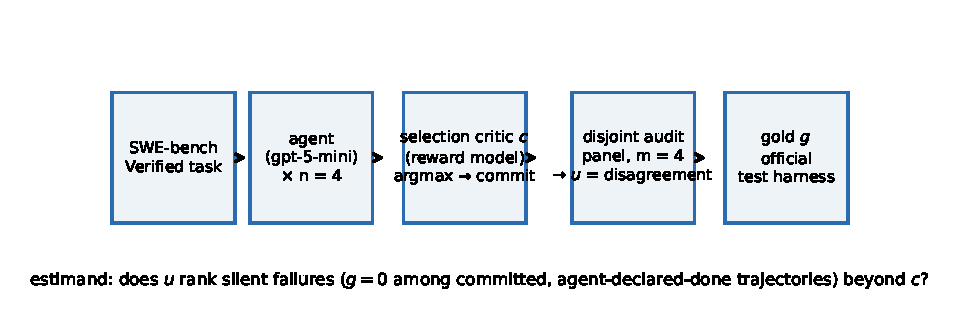
\includegraphics[width=\linewidth]{figures/fig_design.pdf}
\caption{The design. $c$ is the selecting critic's scalar score of a whole trajectory; best-of-$n$ commits the argmax. A disjoint panel of $m$ reward models produces $u$, the sample standard deviation of their rank-normalized scores (rank norms fit on training repositories only). Gold $g$ is the official SWE-bench harness verdict on the committed patch.}\label{fig:design}\end{figure}

\paragraph{Unit and gold.} The unit is one committed trajectory $\tau$. Gold $g(\tau)\in\{0,1\}$ is trajectory-level task success under the official \texttt{swebench} 5.x harness; failed tests do not imply every step was wrong, and we make no step-level claims. Positive class throughout is failure ($\gzero$).

\paragraph{Selection and audit.} $c_{\mathrm{sel}}$ scores the full committed trajectory text; best-of-$n$ ranks $n$ full candidates by this score and commits the top-1. The audit panel $\{c_1,\ldots,c_m\}$ satisfies $c_{\mathrm{sel}}\notin\{c_i\}$ at checkpoint level; $u$ is their disagreement.

\paragraph{Primary population.} Committed trajectories whose agent exited with a submission and a non-empty patch --- the agent believed it was done. Within it, silent failures are $\gzero$.

\paragraph{Metrics.} M1: $\mathrm{AUROC}(u)$ for silent failure. M2: $\mathrm{AUROC}(-c)$. M3 $= $ M1 $-$ M2 with a repository-clustered bootstrap (4{,}000 resamples, groups resampled with the fitted scores held fixed). A held-out logistic $\DeltaAUROC$ was pre-specified as confirmatory only when $\geq 10$ positives fall in the test split; with 41 instances it never did, and we report raw-score AUROCs as registered.

\paragraph{Pre-registration.} Population, positive class, metrics, predictions and a stopping rule (``fewer than ten positives yields no conclusion in either direction'') were committed to the repository before any gold existed (\texttt{PREREGISTRATION\_SWEBENCH\_PILOT.md}). Each later analysis was added as a dated amendment before its data existed. Every deviation is declared in \S\ref{sec:limits}.

\section{Instrument, and what it took to trust it}\label{sec:instrument}
The pilot runs on a laptop and free GPU tiers: mini-swe-agent 2.4.6 driving \texttt{gpt-5-mini} through the OpenAI API (\$0.02 per trajectory with prompt caching), SWE-bench images under Rosetta in a Colima VM on Apple Silicon, reward models on Metal or on Kaggle's free T4s, and the official harness for gold.

We record three instrument failures because each produced a \emph{uniform} failure rate that looked like a finding, and each was caught only by an oracle control. (i) A sandbox flag hid \texttt{numpy} from the gold harness, scoring every trajectory as a failure; caught because the benchmark's reference solutions are run through the harness first. (ii) An LLM-as-judge selecting critic emitted only three distinct values over 640 candidates, so best-of-16 silently became first-draw: 39 of 40 committed trajectories were identical to the $n{=}4$ run. Selection had never happened in the earlier pilots. (iii) On a fresh VM the harness's image pulls failed on an architecture manifest, yielding 41/41 failures in 499 seconds; caught by the harness's own error count. The rule we adopted: a rate of exactly 0\% or 100\% with suspiciously fast timing is an instrument, not a result.

Two statistical defects in our own code were found and fixed before any real run: a power function that reported $\approx$0.40 ``power'' under the true null, and repository grouping that truncated hyphenated repository names, corrupting the held-out split. Both have regression tests.

\section{Results}
\subsection{The premise holds: selection concentrates silent failures}
\begin{figure}[t]\centering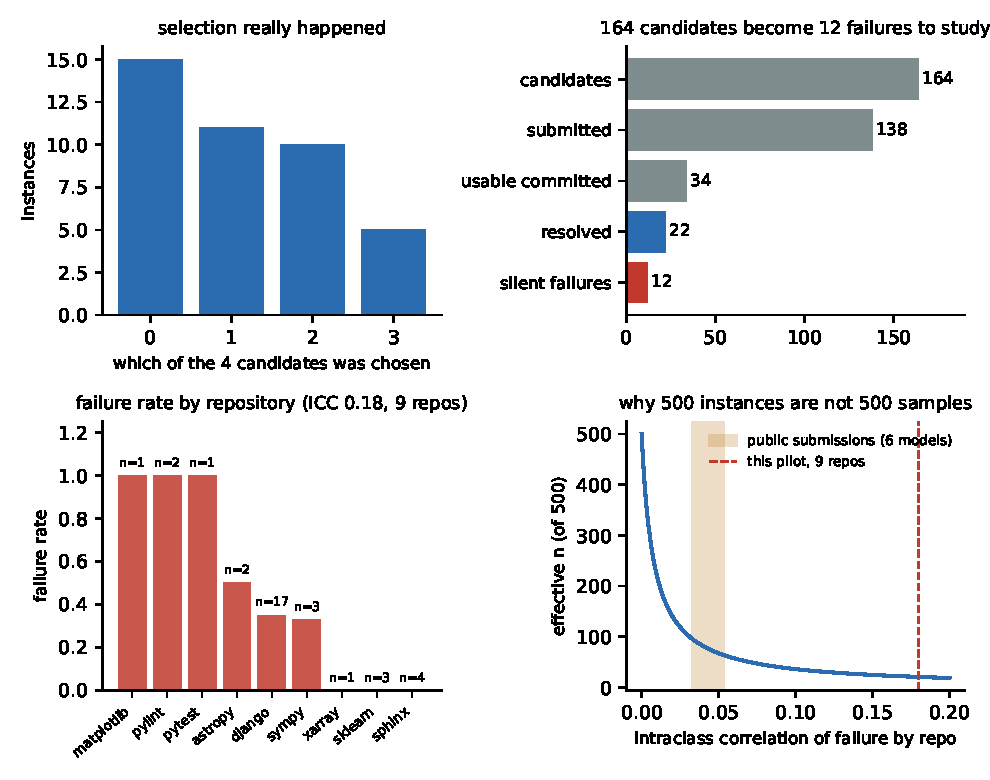
\includegraphics[width=\linewidth]{figures/fig_pilot.pdf}
\caption{The pilot. Top left: best-of-4 with a true reward-model critic genuinely selected (chosen index spread across all four slots; an earlier LLM-judge critic had collapsed to index 0). Top right: from 164 candidates to 12 silent failures. Bottom left: per-repository failure rates, 9 repositories, ICC 0.18. Bottom right: effective sample size on SWE-bench Verified as a function of repository ICC; the public estimate from six leaderboard submissions is 0.033--0.053.}\label{fig:pilot}\end{figure}

Fifty instances were sampled with a fixed seed; generation completed for 41 (the deviation is explained in \S\ref{sec:limits}). Of 164 candidates, 138 submitted a patch (17.7\% hit the 40-step limit or submitted nothing). Selection by \texttt{Skywork-Reward-V2-Qwen3-4B} committed 34 usable trajectories; the harness resolved 22 and failed 12, with zero errors.

\textbf{35.3\% [21.5, 52.1] of committed, agent-declared-complete trajectories were silent failures.} On HumanEval+ the same pipeline yielded 8\% at any selection pressure; SWE-bench supplies the phenomenon in quantity. Selection was real (Fig.~\ref{fig:pilot}, top left), and $\mathrm{corr}(c,u)=0.11$, so $u$ was near-orthogonal to $c$ --- the precondition the design wants.

\subsection{The safeguard does not: the ladder of nulls}
\begin{figure}[t]\centering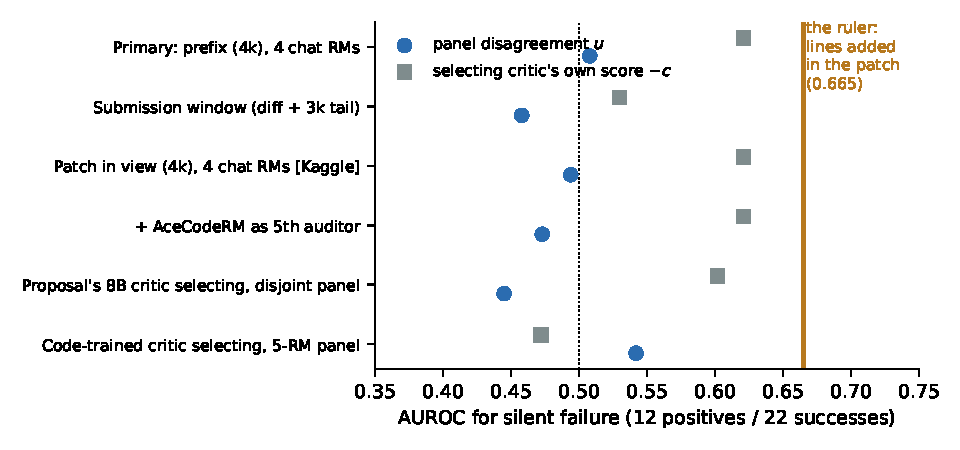
\includegraphics[width=\linewidth]{figures/fig_ladder.pdf}
\caption{Every pre-registered configuration on the same 34 trajectories and 12 positives. Circles: panel disagreement $u$. Squares: the selecting critic's own score. Nothing crosses the ruler.}\label{fig:ladder}\end{figure}

\begin{table}[t]\centering\small
\begin{tabular}{lcccc}\toprule
Configuration & M1 $\mathrm{AUROC}(u)$ & M2 $\mathrm{AUROC}(-c)$ & M3 & 95\% CI \\\midrule
Primary: prefix (4k tok), 4 chat RMs & 0.508 & 0.621 & $-0.114$ & $[-0.37, +0.22]$ \\
\quad robustness, $m{=}3$ (family-disjoint) & 0.545 & 0.621 & $-0.076$ & $[-0.39, +0.23]$ \\
Submission window: diff + last 3k tok & 0.458 & 0.530 & $-0.072$ & $[-0.35, +0.13]$ \\
Patch in view (4k), 4 chat RMs & 0.494 & 0.621 & $-0.127$ & $[-0.28, +0.11]$ \\
\quad + AceCodeRM-7B as 5th auditor & 0.473 & 0.621 & $-0.148$ & $[-0.30, +0.10]$ \\
8B named critic selecting; disjoint panel & 0.445 & 0.602 & $-0.157$ & $[-0.56, +0.14]$ \\
Code-trained critic selecting; 5-RM panel & 0.542 & 0.472 & $+0.069$ & $[-0.21, +0.45]$ \\\bottomrule
\end{tabular}
\caption{The pre-registered primary and all amendments. Same 34 trajectories; 12 positives in every row except the two re-selections (12 and 11). CIs are repository-clustered bootstraps on the paired difference.}\label{tab:ladder}\end{table}

Table~\ref{tab:ladder} and Fig.~\ref{fig:ladder} are the paper. The primary analysis --- four chat-preference reward models auditing a 4{,}096-token prefix --- gave $\mathrm{AUROC}(u)=0.508$. Every subsequent amendment was declared before its data existed and asked whether some specific limitation of that primary was hiding the signal:

\begin{itemize}[leftmargin=1.2em,itemsep=1pt]
\item \emph{The critics never saw the patch.} Scoring the final diff plus the last 3{,}000 tokens: $u$ fell to 0.458.
\item \emph{The critics were too small, or the wrong ones.} Six chat-preference RMs from 1B to 8B, including the proposal's named critic \texttt{Skywork-Reward-V2-Llama-3.1-8B}, each scored with the patch in view: as individual detectors of the 12 known silent failures they scored 0.45--0.64, five of six at or below chance; the panel gave 0.494.
\item \emph{Selection was by the wrong critic.} Re-selecting with the named 8B critic changed 20 of 34 committed trajectories; graded, the failure rate was again 35\%, and $u$ was 0.445.
\item \emph{Chat-preference training is the problem.} \texttt{AceCodeRM-7B}, trained on code with execution-feedback preferences, scored \textbf{0.405} as a detector --- below chance --- and adding it to the panel left $u$ at 0.473. As a selector it changed 24 of 34 trajectories; $u$ on that set was 0.542, its own score 0.472.
\end{itemize}

Each amendment's prediction failed. The confidence intervals on M3 are wide --- twelve positives --- and a moderate positive effect is not excluded by any single row. But seven point estimates, six of them negative, on the same trajectories, under every variation of input, size, identity, training signal and selection regime, do not describe a detector that is merely underpowered. They describe one that is not there.

\subsection{A ruler beats the critics}
\begin{figure}[t]\centering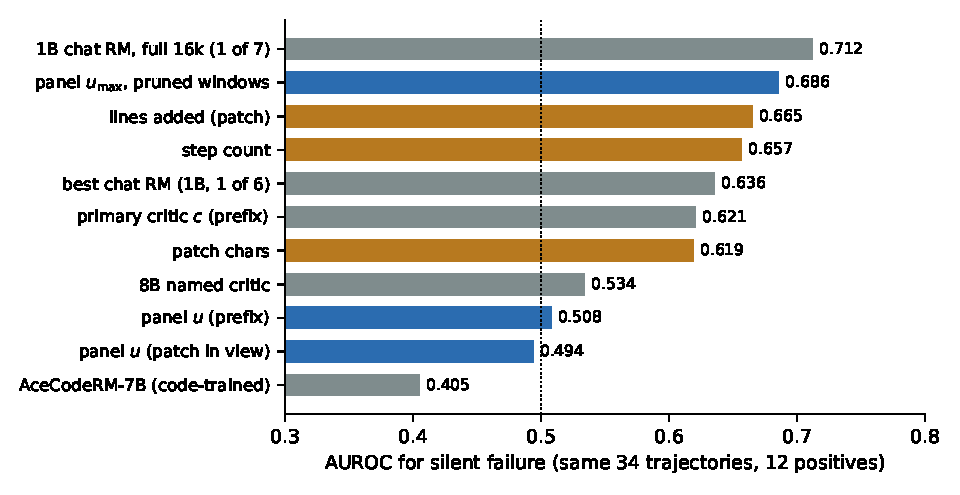
\includegraphics[width=\linewidth]{figures/fig_ruler.pdf}
\caption{Same 34 trajectories, same 12 positives. Gold bars need no model. Exploratory (declared as such): the covariates were registered as controls, not baselines.}\label{fig:ruler}\end{figure}

Two integers, read off the diff and the transcript with no model at all, rank silent failures better than any critic tested (Fig.~\ref{fig:ruler}): lines added in the patch, 0.665; agent step count, 0.657. Bigger patches and longer trajectories fail more. The paired gap over $u$ is $+0.16$ [$-0.11$, $+0.36$] --- a point estimate on twelve positives, and an exploratory one. It is nonetheless the sharpest fact in the study: the critics are not merely failing to add signal beyond selection; they add less than patch size. We propose it as the baseline any future audit critic must clear.

\section{Mechanism: these critics do not hold a judgment}
\begin{figure}[t]\centering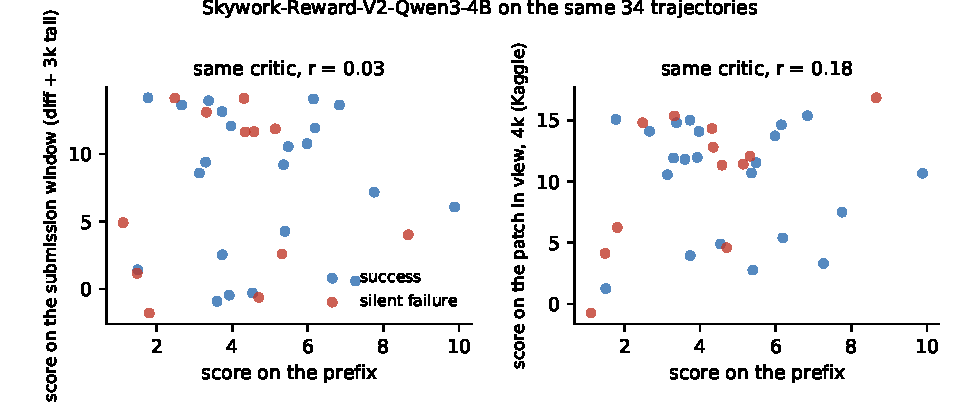
\includegraphics[width=\linewidth]{figures/fig_instability.pdf}
\caption{The primary selecting critic's score on the trajectory prefix (x) against its score on two other windows of the same trajectory (y). Same model, same trajectory, nearly unrelated numbers.}\label{fig:instab}\end{figure}

Fig.~\ref{fig:instab} is why the ladder is flat. The same reward model, given the prefix of a trajectory and then its submission window, produces scores that correlate at 0.03; prefix against the 4k patch-in-view window, 0.18. A critic with a stable view of solution quality would agree with itself. These do not. The modest 0.62 the primary critic achieved on the prefix is therefore best read not as a judgment of the solution --- the prefix contains no solution --- but as a \emph{difficulty} signal from the problem statement: harder-looking problems fail more. Once the input is the solution, that signal disappears and nothing replaces it.

This explains the earlier false positive too. On HumanEval+ with an LLM-as-judge critic, we briefly observed $u=0.69$ and a ``Goodhart signature'' of the critic below chance. Both were artifacts of a critic with three output values on three positives; with a real reward model selecting, both vanished. We withdrew the claim in the record before running the SWE-bench pilot.

\section{Limitations and declared deviations}\label{sec:limits}
\begin{itemize}[leftmargin=1.2em,itemsep=1pt]
\item \textbf{Twelve positives.} Every inference is at the pre-registered eligibility floor. CIs are wide; the argument rests on consistency across configurations, not on any one.
\item \textbf{41 instances, not 50.} Generation stalled at instance 41 when macOS swap exhausted the host disk. The missing nine were determined by list order and the time of the stall, not by the instances.
\item \textbf{Repository clustering.} SWE-bench Verified is 500 instances over 12 repositories, django 46\%. From six public submissions on this scaffold the ICC of failure by repository is 0.033--0.053, giving an effective $n$ of 64--95 of 500 (Fig.~\ref{fig:pilot}); on our 9 repositories it is 0.18. \emph{The cross-repository generalization claim in the original proposal is not testable on this benchmark at any $n$.} We report repository-clustered intervals and make no cross-repository claim.
\item \textbf{Input length.} The primary scored a 4k prefix. The Kaggle amendment targeted 16k but the T4s fell back to 4k on most rows (head 1k + tail 3k, patch included); this is declared per row. \pending{L4 run at true 16k for critics $\leq$4B; larger critics fall back to 8k.}
\item \textbf{Critic classes.} Six chat-preference RMs and one code-trained RM. The 32B code-trained model did not fit a 24 GB GPU. Frontier LLMs as judges with the patch in view were not tested.
\item \textbf{One agent, one task family.} gpt-5-mini at 40 steps on Verified. Silent-failure structure may differ for stronger agents or other benchmarks.
\item \textbf{Windowed auditing.} \pending{Amendment 3 --- structural pruning + overlapping windows, $u_{\max}$, pre-registered against the bar of 0.665. The one structural variant of the panel not yet reported.}
\end{itemize}

\section{Related work}
\todo{Port citations from the proposal's bibliography: Goodhart/winner's curse under best-of-$n$ (Gao et al.\ 2023; inference-time reward hacking), reward-model overoptimization, process reward models and Math-Shepherd-style step labels, SWE-bench/Verified and mini-swe-agent, RewardBench and the Skywork/GRM/AceCode reward models, and negative-result and registered-report precedents in ML evaluation.} The nearest prior work studies critic disagreement as uncertainty for \emph{unselected} outputs; to our knowledge no prior evaluation reports a held-out, selection-conditional, beyond-score test with a disjoint audit panel on agent trajectories with executed gold.

\section{Conclusion}
The premise of critic-audited agents is sound: a third of what a reward-model critic confidently committed on SWE-bench was broken. The proposed safeguard --- disagreement among a disjoint panel of reward models --- did not detect those failures under any configuration we could pre-register and run, and the reason is legible in the data: the critics do not carry a stable signal about code correctness at any input size. Anyone building an audit panel from off-the-shelf reward models should first check whether it beats counting the lines in the patch. Ours did not.

\appendix
\section{Chronology and cost}
\small
\begin{tabular}{lll}\toprule
Stage & What & Cost \\\midrule
Freezes, defects, calibrated power & 18 regression tests & \$0 \\
HumanEval+ pilots 1--3b (instrument validation) & 40 tasks, $n\in\{4,16\}$, 2 judges $\to$ 4 RMs $\to$ RM selection & \$0 \\
SWE-bench infrastructure without admin rights & Colima + Rosetta + swebench 5.x; three oracle controls & \$0 \\
SWE-bench pilot & 164 gpt-5-mini candidates, 41 instances, official gold & \$3.65 \\
Amendment 1 (submission window) & local, 5 RMs & \$0 \\
Amendment 2 (Kaggle 2$\times$T4) & 7 critics, 164 candidates, two re-selections graded & \$0 \\
Amendment 3 (L4) & \pending{} & \$0 \\\bottomrule
\end{tabular}

\section{Reproducibility}
Code, pre-registrations with amendments, every scored row, every critic's scores, the harness reports and the research log are in the repository (\texttt{UPDATES.md} has one entry per stage: done / learned / changed). All figures are generated by \texttt{paper/make\_figures.py} from committed JSON.
\end{document}
